\chapter{Relations Between Two Continuous Variables}

So far we have been dealing with problems where only one variable is measured. Expressions or functions which only depend on one variable are sometimes called "univariate"\index{general}{univariate}. If more than one variable is involved, we are dealing with "multivariate"\index{general}{multivariate} problems. In the simplest case we have two variables involved, and we need a "bivariate"\index{general}{bivariate} data analysis.

For two related variables, the "correlation" measures the association between the two variables. In contrast, a "linear regression" is used for the prediction of the value of one variable from another. For the correlation between many variables, you should look into "correlation tables" (nicely implemented in \emph{seaborn}).  And an extension of linear regression to more than two variables brings you into the realm of statistical modeling (\ref{chapter:Models}).

\section{Correlation}

\subsection{Correlation Coefficient} \index{general}{correlation coefficient}

The \gls{correlation} coefficient between two variables answers the question: "Are the two variables related? I.e. if one variable changes, does the other also change?" If the two variables are normally distributed, the standard measure of determining the correlation coefficient, often ascribed to Pearson\index{general}{correlation!Pearson}, is

\begin{equation}\label{eq:pearson}
  r = \frac{\sum\limits_{i=1}^n (X_i - \bar{X})(Y_i - \bar{Y})}{\sqrt{\sum\limits_{i=1}^n (X_i - \bar{X})^2} \sqrt{\sum\limits_{i=1}^n (Y_i - \bar{Y})^2}}
\end{equation}

With the  sample covariance\index{general}{covariance} $s_{xy}$ defined as

\begin{equation}
  s_{xy} = \frac{\sum\limits_{i=1}^n (X_i - \bar{X})(Y_i - \bar{Y})}{n-1}
\end{equation}

and $s_x, s_y$ the sample standard deviations of the $x$ and $y$ values, respectively,  Eq. \ref{eq:pearson} can also be written as

\begin{equation}
  r = \frac{s_{xy}}{s_x \cdot s_y}.
\end{equation}

Pearson's correlation coefficient, sometimes also referred to as "population correlation coefficient" or "sample correlation", can take any value from -1 to +1. Examples are given in Figure \ref{fig:correlation}. Note that the formula for the correlation coefficient is symmetrical between $x$ and $y$ - which is not the case for linear regression!

\subsection{Rank Correlation}\index{general}{rank correlation}

If the data distribution is not normal, a different approach is necessary. In that case one can rank the set of subjects for each variable and compare the orderings. There are two commonly used methods of calculating the rank correlation. \index{general}{correlation!Spearman}
\index{general}{correlation!Kendall's $\tau$}

\begin{description}
  \item[Spearman's $\rho$], which is exactly the same as the Pearson correlation coefficient $r$ calculated on the ranks of the observations.
  \item[Kendall's $\tau$] is also a rank correlation coefficient, measuring the association between two measured quantities. It is harder to calculate than Spearman's rho, but it has been argued that confidence intervals for Spearman’s rho are less reliable and less interpretable than confidence intervals for Kendall’s tau-parameters.
\end{description}

%\begin{itemize}
%  \item   "Regression to the mean"
%  \item   [xxx Partial correlation (comment) xxx]
%\end{itemize}

%(Lecture 11)

\section{Regression} \index{general}{regression}

\subsection{General linear regression model}

We can use the method of \gls{linreg} when we want to predict the value of one variable from the other.

\begin{figure}
  \centering
  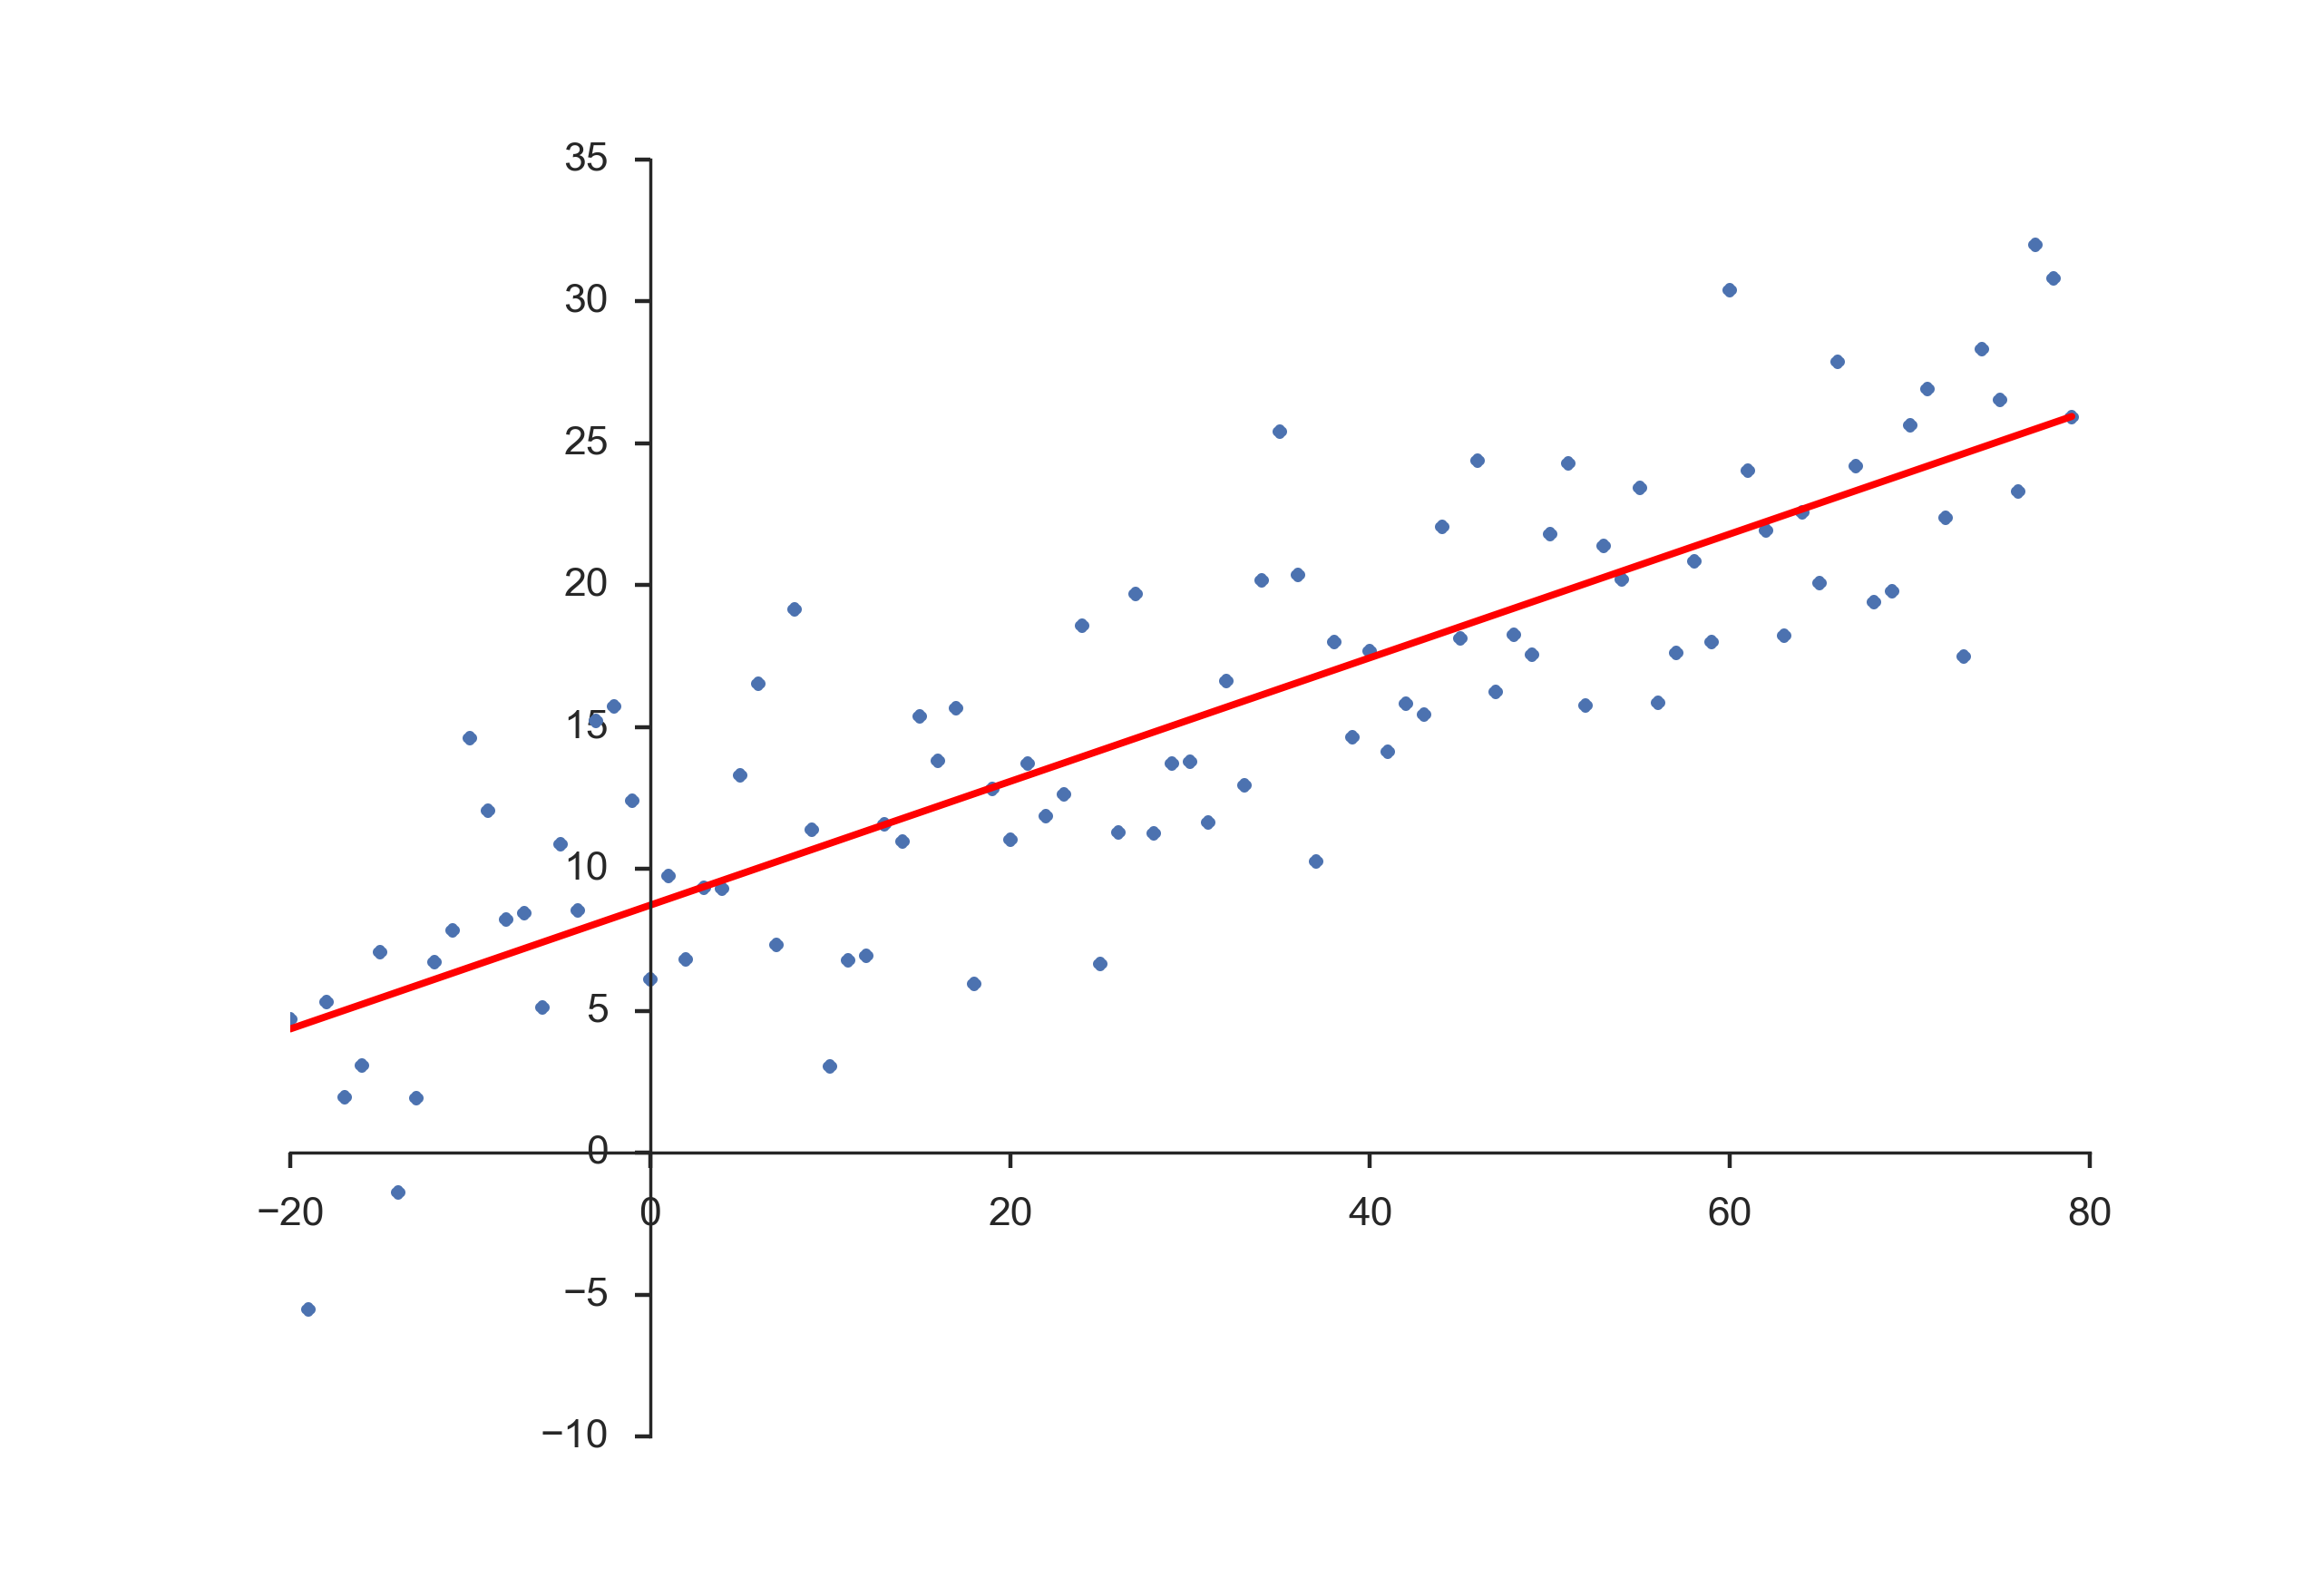
\includegraphics[width=0.75\textwidth]{../Images/Linear_regression.png}\\
  \caption{Linear regression.}\label{fig:regression}
\end{figure}

When we search for the best-fit line to a given $(x_i,y_i)$ dataset, we are looking for the parameters $(k,d)$ which minimize the sum of the squared residuals $\epsilon_i$ in

\begin{equation}\label{eq:simpleRegression}
  y_i = k * x_i + d + \epsilon_i
\end{equation}

where $k$ is the slope or inclination of the line, and $d$ the "intercept". This is in fact just the one-dimensional example of the more general technique, which is described in the next section.
Note that in contrast to the correlation, this relationship between $x$ and $y$ is no more symmetrical: it is assumed that the $x-$values are known exactly, and that all the variability lies in the residuals.

\subsection{Simple Regression}

Suppose there are 7 data points $\left\{ {{y_i},{x_i}} \right\}$, where $i=1,2,…,7$. The simple linear regression model is

\begin{equation}
  y_i = \beta_0 + \beta_1 x_i +\epsilon_i, \,
\end{equation}

where $\beta_0$ is the y-intercept and $\beta_1$ is the slope of the regression line. This model can be represented in matrix form as

\begin{equation}\label{eq:simpleRegressionMatrix}
  \begin{bmatrix}y_1 \\ y_2 \\ y_3 \\ y_4 \\ y_5 \\ y_6 \\ y_7 \end{bmatrix}
  =
  \begin{bmatrix}1 & x_1  \\1 & x_2  \\1 & x_3  \\1 & x_4  \\1 & x_5  \\1 & x_6 \\ 1 & x_7  \end{bmatrix}
  \begin{bmatrix} \beta_0 \\ \beta_1  \end{bmatrix}
  +
  \begin{bmatrix} \epsilon_1 \\ \epsilon_2 \\ \epsilon_3 \\ \epsilon_4 \\ \epsilon_5 \\ \epsilon_6 \\ \epsilon_7 \end{bmatrix}
\end{equation}
where the first column of ones in the matrix on the right hand side represents the y-intercept term while the second column is the x-values associated with the y-value.

\subsection{Design Matrix}


\subsubsection{Quadratic Fit}

The equation for a quadratic fit to the given data is

\begin{equation}
  y_i = \beta_0 + \beta_1 x_i + \beta_2 x_i^2 +\epsilon_i, \,
\end{equation}

This can be rewritten in matrix form:

\begin{equation}\label{eq:polynomialRegression}
  \begin{bmatrix}y_1 \\ y_2 \\ y_3 \\ y_4 \\ y_5 \\ y_6 \\ y_7 \end{bmatrix}
  =
  \begin{bmatrix}1 & x_1 & x_1^2 \\1 & x_2  & x_2^2 \\1 & x_3  & x_3^2 \\1 & x_4  & x_4^2 \\1 & x_5  & x_5^2 \\1 & x_6  & x_6^2 \\ 1 & x_7  & x_7^2 \end{bmatrix}
  \begin{bmatrix} \beta_0 \\ \beta_1  \\ \beta_2 \end{bmatrix}
  +
  \begin{bmatrix} \epsilon_1 \\ \epsilon_2 \\ \epsilon_3 \\ \epsilon_4 \\ \epsilon_5 \\ \epsilon_6 \\ \epsilon_7 \end{bmatrix}
\end{equation}

\subsubsection{General Formulation}

In general, this can be rewritten in matrix form as:

\begin{equation}\label{eq:DesignMatrix}
    \mathbf{y} = \mathbf{X} \cdot \mathbf{\beta } + \mathbf{\varepsilon }
\end{equation}

$\mathbf{y}$ is a vector of dimension $(n \times 1)$ and is called the Endogenous Variable, the Design Matrix \index{general}{design matrix} $\mathbf{X}$ is a matrix of dimension $(n \times k)$ where each column is an explanatory variable, and $\mathbf{\varepsilon }$ is the error term, the elements of which are assumed to be normally distributed about zero. $\mathbf{\beta }$ is the vector of dimension $(k \times 1)$ and contains the parameters we want to estimate.

% [xxx "the elements of which are assumed to be normally distributed about zero" - is this what the reviewer wanted, when he/she said "No, we also want variance of epsilon" xxx]
\subsection{Coefficient of determination}

In order to interpret r, let me first define a few common terms.

\begin{description}
  \item[Residuals] \index{general}{residuals}Differences between observed values and predicted values.
\end{description}

\begin{figure}
  \centering
  \includegraphics[width=0.75\textwidth]{../Images/residuals_linreg.png}\\
  \caption{Best-fit linear regression line (red) and residuals (black). }\label{fig:residuals}
\end{figure}

A data set has values $y_i$, each of which has an associated modelled value $f_i$ (also sometimes referred to as $\hat{y}_i$). Here, the values $y_i$ are called the Observed Values, and the modelled values $f_i$ are sometimes called the Predicted Values.

In the following $\bar{y}$ is the mean of the observed data:

\begin{equation}
  \bar{y}=\frac{1}{n}\sum_{i=1}^n y_i
\end{equation}

where n is the number of observations.

The "variability" of the data set is measured through different sums of squares:

\vspace{5 mm}

    $SS_\text{tot}=\sum_i (y_i-\bar{y})^2$, the total sum of squares (proportional to the sample variance);

    $SS_\text{mod}=\sum_i (f_i -\bar{y})^2$, the sum of squares of the model values, also called the explained sum of squares;

    $SS_\text{res}=\sum_i (y_i - f_i)^2\,$, the sum of squares of residuals, also called the residual sum of squares.

\vspace{5 mm}

The notations $SS_{R}$ and $SS_{E}$ should be avoided, since in some texts their meaning is reversed to "Residual sum of squares" and "Explained sum of squares", respectively.

\begin{figure}
  \centering
  \includegraphics[width=0.75\textwidth]{../Images/Coefficient_of_Determination.png}\\
  \caption{The better the linear regression (on the right) fits the data in comparison to the simple average (on the left graph), the closer the value of $R^2$ is to one. The areas of the blue squares represent the squared residuals with respect to the linear regression. The areas of the red squares represent the squared residuals with respect to the average value (from Wikipedia)}\label{fig:CoefDetermination}
\end{figure}

\vspace{5 mm}

With these expressions, the most general definition of the coefficient of determination, $R^2$, is

\begin{equation}\label{eq:R2}
  R^2 \equiv 1 - {SS_{\rm res}\over SS_{\rm tot}}.\,
\end{equation}

Since

\begin{equation}
  SS_\text{tot} = SS_\text{mod} + SS_\text{res}
\end{equation}

Eq. \ref{eq:R2} is equivalent to

\begin{equation}
  R^2 = \frac{SS_\text{mod}}{SS_\text{tot}}
\end{equation}

For simple linear regression (i.e. line-fits), the coefficient of determination\index{general}{coefficient of determination} or $R^2$ is the square of the correlation coefficient $r$. It is easier to interpret than the correlation coefficient r: values of $R^2$ close to 1 are good, values close to 0 are poor.
Note that for general models it is common to write $R^2$, whereas for simple linear regression $r^2$ is used.

\subsubsection{Relation to unexplained variance}\index{general}{unexplained variance}

In a general form, $R^2$ can be seen to be related to the unexplained variance, since the second term in Eq. \ref{eq:R2} compares the unexplained variance (variance of the model's errors) with the total variance (of the data).

\begin{figure}
  \centering
  \includegraphics[width=0.75\textwidth]{../Images/Correlation_examples2.png}\\
  \caption{Several sets of (x, y) points, with the correlation coefficient of x and y for each set. Note that the correlation reflects the non-linearity and direction of a linear relationship (top row), but not the slope of that relationship (middle), nor many aspects of nonlinear relationships (bottom). N.B.: the figure in the center has a slope of 0 but in that case the correlation coefficient is undefined because the variance of Y is zero. (In Wikipedia. Retrieved May 27, 2015, from http://en.wikipedia.org/wiki/Correlation\_and\_dependence)}\label{fig:correlation}
\end{figure}

\subsubsection{Examples}

How large $R^2$ must be to be considered good depends on the discipline. They are usually expected to be larger in the physical sciences than it is in biology or the social sciences. In finance or marketing, it also depends on what is being modeled.

Caution: the sample correlation and $R^2$ are misleading if there is a nonlinear relationship between the independent and dependent variables!


\subsection{Coding}

If you have vectors $x,y$ containing your data, you can use \texttt{statsmodels} to create a design matrix that also includes the $1's$ for the offset:

\begin{lstlisting}[language=Python]
    import statsmodels.api as sm
    Xmat = sm.add_constant(x)
\end{lstlisting}

The parameters are then easily found as

\begin{lstlisting}[language=Python]
    params = np.linalg.lstsq(Xmat, y)
\end{lstlisting}

However, you get a lot more information if you use the OLS-fit from \texttt{statmodels}:

\begin{lstlisting}[language=Python]
    import numpy as np
    import statsmodels.api as sm

    # Generate artificial data
    nobs = 100
    X = np.random.random(nobs)
    X = sm.add_constant(X)
    beta = [5, 3.5]
    e = np.random.random(nobs)
    y = np.dot(X, beta) + e

    # Fit regression model
    results = sm.OLS(y, X).fit()

    # Inspect the results
    print(results.summary())
\end{lstlisting}

yields the following results:

\begin{lstlisting}[language=Python]
                            OLS Regression Results
==============================================================================
Dep. Variable:                      y   R-squared:                       0.923
Model:                            OLS   Adj. R-squared:                  0.922
Method:                 Least Squares   F-statistic:                     1173.
Date:                Fri, 04 Jul 2014   Prob (F-statistic):           2.45e-56
Time:                        14:49:08   Log-Likelihood:                -15.390
No. Observations:                 100   AIC:                             34.78
Df Residuals:                      98   BIC:                             39.99
Df Model:                           1
==============================================================================
                 coef    std err          t      P>|t|      [95.0% Conf. Int.]
------------------------------------------------------------------------------
const          5.4410      0.059     92.685      0.000         5.324     5.557
x1             3.5718      0.104     34.250      0.000         3.365     3.779
==============================================================================
Omnibus:                       21.620   Durbin-Watson:                   2.302
Prob(Omnibus):                  0.000   Jarque-Bera (JB):                5.798
Skew:                           0.223   Prob(JB):                       0.0551
Kurtosis:                       1.908   Cond. No.                         4.60
==============================================================================
\end{lstlisting}

The meaning of many of these parameters is described in the chapter \nameref{chapter:Models}.

From the \texttt{results}, you can extract e.g. the model parameters, standard errors, confidence intervals, and residuals:

\begin{lstlisting}[language=Python]
    params = results.params
    std_err = results.bse
    ConfInt = results.conf_int()
    residuals = results.resid
\end{lstlisting}

\subsection{Assumptions}

To use the technique of linear regression, the following assumptions should be fulfilled:

\begin{enumerate}
  \item The independent variables (i.e. $x$) are exactly known.
  \item Validity. Most importantly, the data you are analyzing should map to the research question you are trying to answer. This sounds obvious but is often overlooked or ignored because it can be inconvenient. For example, a linear regression does not properly describe a quadratic curve.
  \item Additivity and linearity. The most important mathematical assumption of the regression model is that its deterministic component is a linear function of the separate predictors.
  \item Independence of errors from the values of the independent variables.
  \item Equal variance of errors.
  \item Normality of errors.
\end{enumerate}

\begin{figure}
  \centering
  \includegraphics[width=0.75\textwidth]{../Images/Anscombes_quartet.png}\\
  \caption{The sets in the "Anscombe's quartet"\index{general}{Anscombe's quartet} have the same linear regression line but are themselves very different.}
\end{figure}

\PyImg "multivariate.py" (p \pageref{py:multivariate}): Analysis of multivariate data (regression, correlation).
\index{python}{multivariate}

\begin{figure}
  \centering
  \includegraphics[width=0.75\textwidth]{../Images/regression_wLegend.png}\\
  \caption{Regression, with confidence intervals for the mean, as well as for the predicted data. The red dotted line shows the confidence interval for the mean; and the green dotted line the confidence interval for predicted data. (This can be compared to the standard error and the standard deviation for a population.) The corresponding code can be found
  at p. \pageref{py:fitLine}} \label{fig:regline}
\end{figure}

Since to my knowledge there exists no program in the \emph{Python} standard library (or numpy, scipy) to calculate the confidence intervals for a regression line, I include my corresponding program \emph{lineFit.py} \ref{py:fitLine}. The output of this program is shown in Figure \ref{fig:regline}. This program also shows how \emph{Python} programs intended for distribution should be documented.

\PyImg "fitLine.py" (p \pageref{py:fitLine}): Linear regression fit.
\index{python}{fitLine}

\section{Exercises}

\begin{enumerate}
  \item \textbf{Correlation}

    Read in the data for the average yearly temperature at the Sonnblick, from     \emph{https://github.com/thomas-haslwanter/statsintro/blob/master/Data/data\_others/AvgTemp.xls}
    Calculate the Pearson and Spearman correlation, and Kendall's tau, for the temperature vs. year.

  \item \textbf{Regression}

    For the same data, calculate the yearly increase in temperature, assuming a linear increase with time.
    Is this increase significant?

  \item \textbf{Normality Check}

    For the data from the regression model, check if the model is ok by testing if the residuals are normally distributed (e.g. by using the Kolmogorov-Smirnov test)

\end{enumerate}


